\chapter{Estudo de Caso }
% : Requisitos, Organização, Métodos, Design, Implementação e Testes
\label{cap:estudo_caso}
Este capítulo apresenta o contexto, os requisitos, a organização, os métodos, o design, a implementação e os testes realizados no desenvolvimento do estudo de caso em uma plataforma de notícias sobre tecnologia chamada WallTech.

\section{Contexto}
\label{section:contexto}
Este estudo de caso é realizado em uma empresa fictícia do setor de notícias sobre tecnologia, com foco em fornecer conteúdos atualizados e relevantes sobre inovações e tendências. O público-alvo inclui entusiastas de tecnologia, profissionais da área e usuários que desejam acompanhar novidades do setor, podendo acessar a plataforma em dispositivos móveis ou computadores graças ao design responsivo.

Para a análise, foram desenvolvidos dois protótipos da aplicação, um utilizando \acrfull{csr} com React e outro utilizando \acrfull{ssr} com Next.js, com o objetivo de comparar o desempenho, a interatividade e o \english{\acrfull{seo}} de cada abordagem.

A Figura \ref{fig:caso-uso-walltech} apresenta o diagrama de caso de uso da plataforma, mostrando as principais funcionalidades disponíveis para o usuário anônimo. O diagrama ilustra as interações do usuário com o sistema, permitindo que ele visualize a lista de notícias mais recentes, acesse os detalhes de uma notícia ao clicar nela ou realize buscas específicas utilizando palavras-chave.  

\begin{figure}[H]
  \centering
  \caption{Diagrama de caso de uso}
  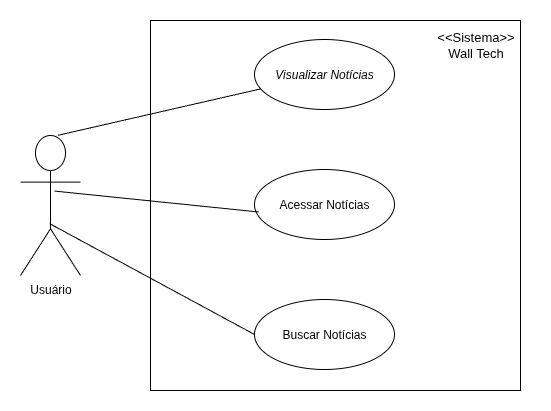
\includegraphics[width=0.7\textwidth]{media/wall_tech_use_case.png}
  \legend{Fonte: os autores.}
  \label{fig:caso-uso-walltech}
\end{figure}


\section{Processo de Desenvolvimento}
\label{section:processo-desenvolvimento}
O processo de desenvolvimento utilizado para construir a plataforma WallTech segue a metodologia ágil \english{Kanban}. Essa metodologia de desenvolvimento ágil é baseada em um quadro de tarefas, no qual cada tarefa é representada por um cartão \cite{gomes2014kanban}. O quadro Kanban é dividido em colunas que representam o estado atual de cada tarefa. As colunas mais comuns são: \english{To Do}, \english{In Progress} e \english{Done}, e o quadro é atualizado conforme as tarefas são realizadas. Além dessas colunas, o processo foi adaptado para incluir colunas adicionais como \english{Docs} e \english{Test}, permitindo que a documentação e os testes fossem gerenciados de forma organizada e eficiente durante o desenvolvimento.

A Figura \ref{fig:kanban-walltech} apresenta um exemplo do quadro Kanban utilizado no \english{GitHub Projects}, mostrando a organização das tarefas e o progresso do desenvolvimento da plataforma WallTech. O quadro reflete a estrutura de colunas adaptada, proporcionando uma visão clara do fluxo de trabalho da equipe, o que facilita o acompanhamento das tarefas em diferentes estágios.

Após a definição das funcionalidades principais do sistema, as tarefas foram inicialmente documentadas como \english{user stories}. As \english{user stories} são descrições simples e compreensíveis das funcionalidades a serem implementadas, permitindo uma comunicação clara entre a equipe de desenvolvimento e as partes interessadas. Cada \english{user story} é associada a um conjunto de requisitos específicos e uma definição de pronto, facilitando a compreensão do que precisa ser desenvolvido.

A partir dessas \english{user stories}, as \english{issues} foram criadas no \english{GitHub Projects}. Cada \english{issue} representa uma tarefa específica que deve ser realizada, baseada nas \english{user stories}. No \english{GitHub Projects}, essas \english{issues} são organizadas nas colunas do quadro Kanban, permitindo que a equipe visualize o progresso de cada tarefa e as mova conforme o andamento do trabalho.

A Figura \ref{fig:kanban-userstories} mostra um exemplo de cartão \english{issue} no \english{GitHub Projects}, ilustrando como as \english{user stories} são transformadas em tarefas e organizadas dentro do quadro Kanban. Cada \english{issue} possui detalhes sobre a tarefa, como descrições, prioridade e prazo, facilitando o gerenciamento e a execução das atividades no time de desenvolvimento.

\begin{figure}[H]
  \centering
  \caption{Exemplo de quadro Kanban no \english{GitHub Projects}}
  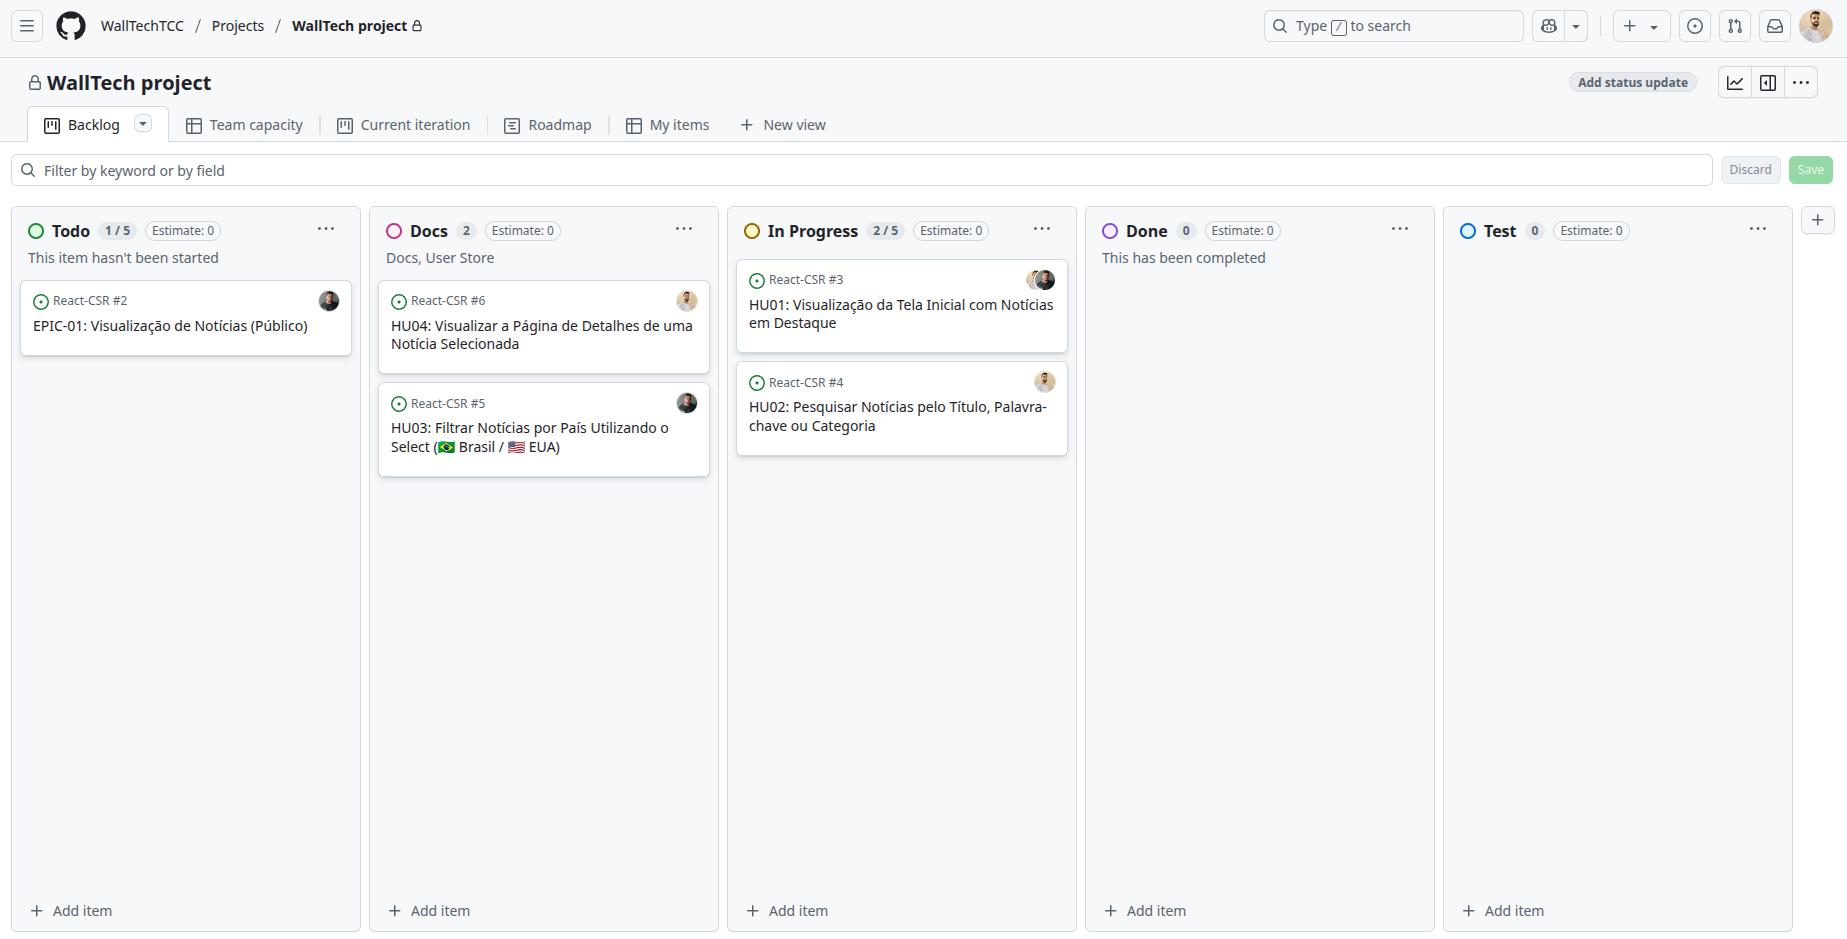
\includegraphics[width=1.0\textwidth]{media/wall_tech_kanban.png}
  \legend{Fonte: os autores.}
  \label{fig:kanban-walltech}
\end{figure}

\begin{figure}[H]
  \centering
  \caption{Exemplo de cartão \english{issue} no \english{GitHub Projects}}
  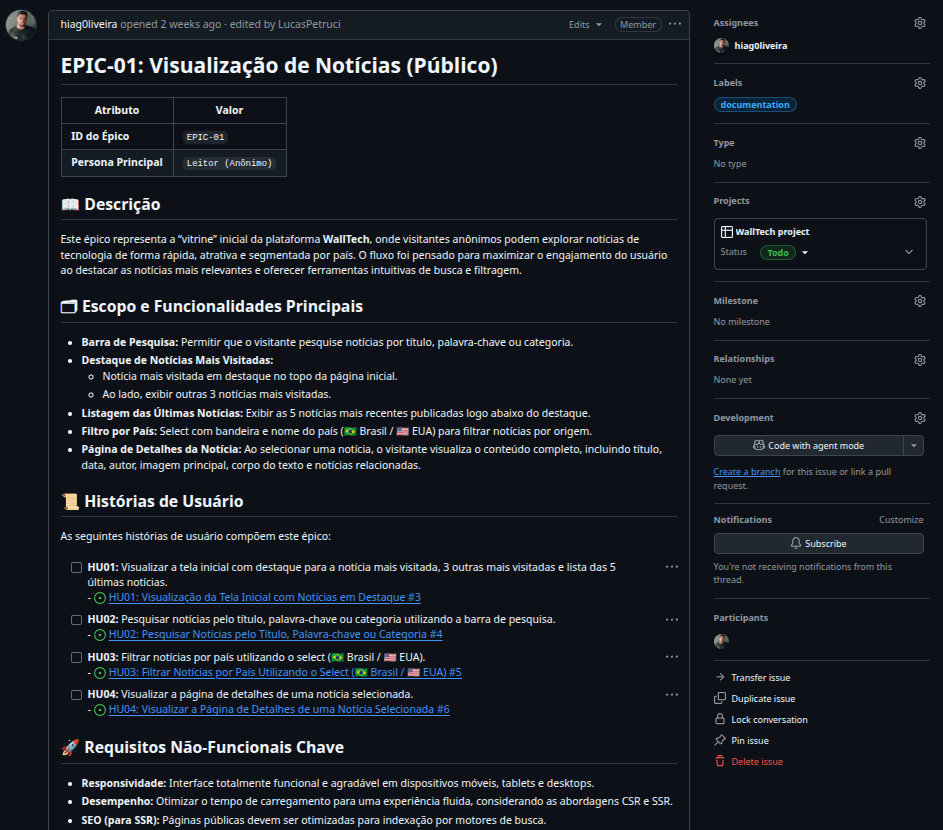
\includegraphics[width=0.7\textwidth]{media/wall_tech_epic.png}
  \legend{Fonte: os autores.}
  \label{fig:kanban-userstories}
\end{figure}




\subsection{Planejamento Funcional: Épico e Histórias de Usuário}

Para guiar o desenvolvimento da plataforma \textbf{WallTech}, foi adotada uma abordagem baseada em práticas ágeis, especialmente no uso de \textit{épicos} e \textit{histórias de usuário}. Essa técnica visa descrever funcionalidades a partir da perspectiva do usuário, proporcionando clareza sobre o propósito e os objetivos de cada componente da aplicação.

As histórias de usuário foram redigidas segundo o modelo dos \textbf{3Ws (Who, What, Why)}, uma técnica comum em análise de requisitos que busca responder:
\begin{itemize}
  \item \textbf{Who (Quem):} Quem está solicitando ou interagindo com a funcionalidade?
  \item \textbf{What (O quê):} Qual é a ação ou funcionalidade desejada?
  \item \textbf{Why (Por quê):} Qual é o benefício ou valor esperado para o usuário?
\end{itemize}

Esse modelo torna a narrativa mais centrada no usuário e contribui para um entendimento compartilhado entre desenvolvedores, designers e partes interessadas. Além disso, as funcionalidades foram agrupadas em \textbf{épicos}, que representam blocos de funcionalidades coesas e de maior escala dentro do sistema.

A seguir, apresenta-se o \textbf{EPIC-01}, responsável por organizar as funcionalidades relacionadas à visualização pública de notícias na plataforma WallTech, seguido de suas respectivas histórias de usuário.

\subsubsection*{EPIC-01: Visualização de Notícias (Público)}

\begin{itemize}
  \item \textbf{ID do Épico:} EPIC-01
  \item \textbf{Persona Principal:} Leitor (Anônimo)
\end{itemize}

\noindent \textbf{Descrição:} Este épico representa a “vitrine” da plataforma WallTech, onde visitantes anônimos podem explorar notícias de tecnologia de forma rápida, atrativa e segmentada por país. O fluxo foi pensado para maximizar o engajamento do usuário ao destacar as notícias mais relevantes e oferecer ferramentas intuitivas de busca e filtragem.

\noindent \textbf{Funcionalidades Principais:}
\begin{itemize}
  \item Barra de pesquisa (por título, palavra-chave ou categoria);
  \item Destaque para a notícia mais visitada e outras três recentemente acessadas;
  \item Listagem das cinco últimas notícias;
  \item Filtro por país (Brasil ou EUA);
  \item Página de detalhes da notícia com conteúdo completo e relacionadas.
\end{itemize}

\noindent \textbf{Requisitos Não-Funcionais:}
\begin{itemize}
  \item Interface responsiva em diferentes dispositivos;
  \item Otimização de desempenho para carregamento rápido;
  \item Suporte a SEO nas páginas públicas (relevante em SSR).
\end{itemize}

\noindent \textbf{Critérios de Aceite:}
\begin{itemize}
  \item Visitantes conseguem navegar e visualizar notícias sem necessidade de login;
  \item É possível realizar pesquisas e aplicar filtros por país;
  \item A navegação é responsiva, intuitiva e eficiente;
  \item A página de detalhes apresenta informações completas da notícia.
\end{itemize}

\subsubsection*{HU01: Visualização da Tela Inicial com Notícias em Destaque}

\begin{itemize}
  \item \textbf{Who:} Visitante anônimo
  \item \textbf{What:} Ver na página inicial uma barra de pesquisa, uma notícia mais visitada em destaque, três outras recém acessadas e uma lista com as cinco últimas notícias publicadas.
  \item \textbf{Why:} Explorar rapidamente o conteúdo mais relevante e recente sobre tecnologia.
\end{itemize}

\noindent \textbf{História:} \textit{Como um visitante, quero ver na página inicial uma barra de pesquisa, a notícia mais visitada em destaque, outras três recém visitadas ao lado e as cinco últimas notícias abaixo, para que eu possa explorar rapidamente o conteúdo mais relevante sobre tecnologia.}

\noindent \textbf{Critérios de Aceite:}
\begin{itemize}
  \item A página inicial contém uma barra de pesquisa funcional;
  \item A notícia mais visitada aparece em destaque;
  \item Outras três notícias aparecem ao lado da principal;
  \item Abaixo, as cinco últimas notícias são exibidas em ordem cronológica;
  \item Interface é responsiva e com bom desempenho.
\end{itemize}

\subsubsection*{HU02: Pesquisar Notícias por Palavra-chave ou Categoria}

\begin{itemize}
  \item \textbf{Who:} Visitante
  \item \textbf{What:} Utilizar a barra de pesquisa para buscar por título, palavra-chave ou categoria.
  \item \textbf{Why:} Encontrar conteúdos relevantes de forma eficiente.
\end{itemize}

\noindent \textbf{História:} \textit{Como um visitante, quero pesquisar notícias por título, palavra-chave ou categoria, para que eu possa encontrar facilmente conteúdos relevantes sem precisar navegar por toda a lista.}

\noindent \textbf{Critérios de Aceite:}
\begin{itemize}
  \item Campo de texto para busca;
  \item Filtro por categoria;
  \item Resultados relevantes são exibidos com base na busca;
  \item A busca pode ser combinada com o filtro por categoria;
  \item Mensagem amigável exibida em caso de nenhum resultado.
\end{itemize}

\subsubsection*{HU03: Filtrar Notícias por País}

\begin{itemize}
  \item \textbf{Who:} Visitante
  \item \textbf{What:} Filtrar as notícias por país usando um seletor com bandeiras.
  \item \textbf{Why:} Visualizar conteúdos específicos da localidade desejada.
\end{itemize}

\noindent \textbf{História:} \textit{Como um visitante, quero filtrar notícias por país (Brasil ou EUA), para que eu possa visualizar apenas conteúdos relevantes para minha localidade ou interesse regional.}

\noindent \textbf{Critérios de Aceite:}
\begin{itemize}
  \item Menu com seleção de país exibindo bandeira e nome;
  \item Lista de notícias é atualizada dinamicamente conforme a seleção;
  \item O filtro mantém o estado ao navegar;
  \item Filtro compatível com busca por palavra-chave ou categoria.
\end{itemize}

\subsubsection*{HU04: Visualizar Detalhes de uma Notícia}

\begin{itemize}
  \item \textbf{Who:} Visitante
  \item \textbf{What:} Acessar a página de detalhes de uma notícia específica.
  \item \textbf{Why:} Ler o conteúdo completo e visualizar informações adicionais.
\end{itemize}

\noindent \textbf{História:} \textit{Como um visitante, quero clicar em uma notícia para acessar sua página de detalhes, para que eu possa ler o conteúdo completo e visualizar informações relacionadas.}

\noindent \textbf{Critérios de Aceite:}
\begin{itemize}
  \item Acesso a uma URL única da notícia;
  \item Exibição completa do conteúdo (título, autor, data, imagem, corpo do texto, país de origem);
  \item Exibição de até três notícias relacionadas;
  \item Página de erro amigável no caso de URL inválida;
  \item Botão para retornar à lista ou pesquisa anterior.
\end{itemize}









\section{Requisitos}
\label{section:requisitos}

O levantamento e a definição dos requisitos da plataforma \textbf{WallTech} foram guiados pelas necessidades dos usuários e organizados por meio da técnica de \textit{histórias de usuário}, agrupadas em \textit{épicos}. A partir da análise funcional do \textbf{EPIC-01 — Visualização de Notícias (Público)}, foram identificadas as principais funcionalidades esperadas para a aplicação, considerando tanto o fluxo de interação do visitante quanto os objetivos de usabilidade, desempenho e escalabilidade.

Os requisitos a seguir foram organizados em duas categorias: \textbf{funcionais}, que representam as funcionalidades diretamente percebidas pelos usuários, e \textbf{não funcionais}, que tratam de atributos como desempenho, acessibilidade e responsividade.

\subsection{Requisitos Funcionais}
\label{subsec:requisitos-funcionais}

\begin{itemize}
  \item O sistema deve permitir que visitantes visualizem uma lista de notícias recentes e em destaque.
  \item O sistema deve disponibilizar uma barra de pesquisa por palavra-chave, título ou categoria.
  \item O sistema deve permitir a filtragem de notícias por país (🇧🇷 Brasil ou 🇺🇸 EUA).
  \item O sistema deve possibilitar o acesso aos detalhes completos de uma notícia selecionada.
  \item O sistema deve armazenar localmente os acessos recentes para melhorar a experiência do usuário.
  \item O sistema deve apresentar mensagens claras em situações de ausência de conteúdo.
\end{itemize}

\subsection{Requisitos Não Funcionais}
\label{subsec:requisitos-nao-funcionais}

\begin{itemize}
  \item A interface deve ser responsiva, adaptando-se corretamente a diferentes tamanhos de tela.
  \item O carregamento das páginas deve ser otimizado, proporcionando uma experiência fluida mesmo em conexões lentas.
  \item O sistema deve estar preparado para indexação por motores de busca (SEO), quando aplicado via Server-Side Rendering.
  \item A navegação deve ser acessível, com suporte a teclado e leitores de tela.
  \item A interface deve manter a consistência visual e funcional entre suas versões SPA e MPA.
\end{itemize}




\section{Design do Sistema}
\label{cap:design}

O design do sistema foi orientado para refletir as diferenças estruturais entre as abordagens \acrshort{spa} e \acrshort{mpa}, levando em consideração os requisitos funcionais da plataforma \textit{WallTech}. Esta vitrine digital exibe notícias de tecnologia obtidas por meio da \textit{NewsAPI}, com recursos de busca, filtragem e destaque de conteúdo segmentado por país. Não há backend próprio, sendo todas as chamadas feitas diretamente para a API externa, o que simplifica a arquitetura e acentua o papel do frontend na renderização de conteúdo.

Para modelagem arquitetural e comportamental, foram utilizados diagramas da UML, incluindo:
\begin{itemize}
  \item \textbf{Diagrama de Caso de Uso}, para representar as principais funcionalidades acessadas pelos usuários visitantes.
  \item \textbf{Diagrama de Sequência}, a fim de ilustrar o fluxo de interação entre navegador e a \textit{NewsAPI} durante operações como busca e carregamento de notícias.
  \item \textbf{Diagrama de Componentes}, para representar os módulos da aplicação, como a interface, o serviço de requisição à API, e os componentes de renderização.
\end{itemize}

As decisões de design foram fundamentadas em boas práticas para renderização web discutidas por \cite{osmani2025}, bem como nas diretrizes da literatura especializada em arquitetura de frontend, como apresentado pela \cite{atori2024}.

Segundo \cite{osmani2025}, a escolha entre renderização no cliente ou no servidor deve considerar o contexto da aplicação, os requisitos de desempenho e os objetivos de SEO. Já o artigo da \cite{atori2024} destaca que SPAs tendem a oferecer maior fluidez e interatividade, enquanto MPAs são mais eficazes em aplicações que dependem de indexação e acessibilidade.

\section{Abordagens de Renderização e Navegação}
\label{section:abordagens-renderizacao}

Para o estudo comparativo, a plataforma foi desenvolvida em duas arquiteturas distintas de renderização e navegação: 
\acrfull{ssr} com \acrfull{mpa} e \acrfull{csr} com \acrfull{spa}.  
Cada abordagem foi implementada com tecnologias adequadas ao seu paradigma — Next.js para \acrshort{ssr}/\acrshort{mpa} e React para \acrshort{csr}/\acrshort{spa} — permitindo observar diferenças de desempenho, interatividade e otimização para mecanismos de busca (\acrshort{seo}).

A seguir, cada abordagem é apresentada com seu fluxo típico de funcionamento, diagrama de componentes (representando a estrutura modular) e diagrama de sequência (detalhando as interações passo a passo).

\subsection{SSR/MPA - Fluxo e Arquitetura}
\label{subsec:ssr-mpa}

Na abordagem \acrfull{ssr} com \acrfull{mpa}, cada página é renderizada no servidor a partir de uma requisição HTTP completa. O HTML final já é entregue com os dados integrados, permitindo que o navegador exiba o conteúdo imediatamente, favorecendo o tempo de carregamento inicial e a indexação por \textit{crawlers} \cite{atori2024}.

\begin{itemize}
  \item O \textbf{usuário} acessa o site;
  \item O \textbf{navegador} envia uma requisição \texttt{GET} ao \textbf{servidor Next.js};
  \item O servidor obtém os dados mais recentes na \textbf{NewsAPI};
  \item O servidor monta a página HTML já com os dados;
  \item O HTML é enviado ao navegador e exibido;
  \item Cada navegação subsequente gera nova requisição completa ao servidor;
  \item Scripts no cliente utilizam \textbf{LocalStorage} para melhorar a experiência.
\end{itemize}
  
A Figura \ref{fig:component-diagram-next} ilustra como, nesta arquitetura, o \textbf{navegador} interage diretamente com o \textbf{Servidor Next.js} para cada página requisitada. O servidor, por sua vez:
\begin{enumerate}
  \item Identifica a rota usando o \textbf{roteamento baseado em arquivos};
  \item Executa a lógica de busca de dados (\texttt{getServerSideProps});
  \item Faz chamadas à \textbf{NewsAPI} para obter o conteúdo;
  \item Renderiza o HTML e o envia ao cliente.
\end{enumerate}

A Figura \ref{fig:sequence-diagram-ssr} detalha a ordem das interações. O usuário inicia a navegação, o servidor processa a requisição, consulta a API externa, renderiza o HTML e envia a resposta pronta para o cliente. O uso de \textit{hydration} ativa a interatividade após o carregamento inicial.

\begin{figure}[H]
  \centering
  \caption{Diagrama de sequência - \acrshort{ssr}/\acrshort{mpa}}
  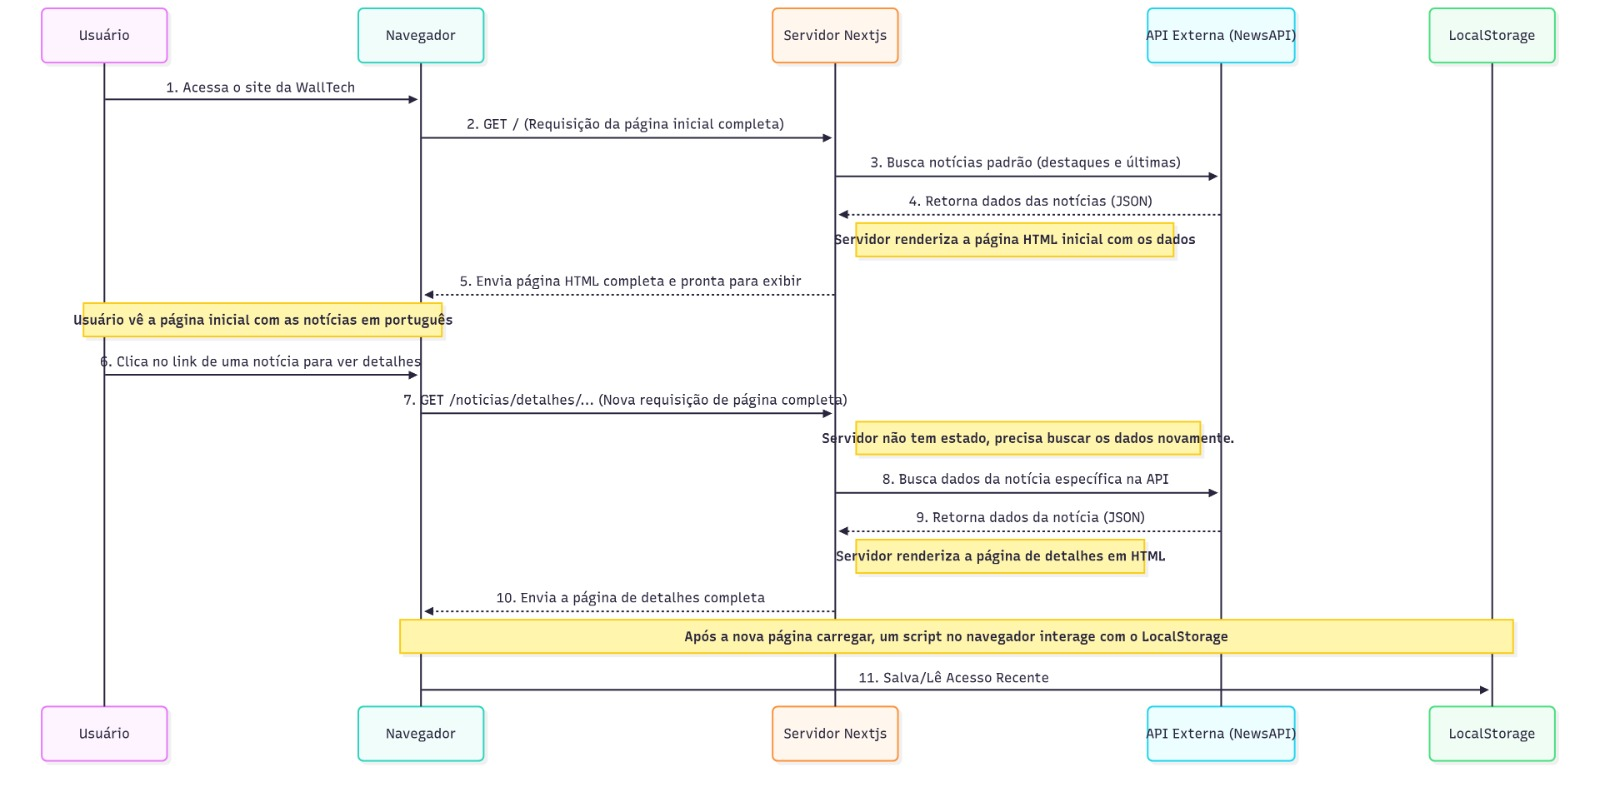
\includegraphics[width=1\textwidth]{media/wall_tech_sequence_diagram.jpeg}
  \legend{Fonte: os autores.}
  \label{fig:sequence-diagram-ssr}
\end{figure}


A Figura \ref{fig:component-diagram-next} mostra que, nessa arquitetura, o \textbf{servidor Next.js} centraliza o roteamento, a obtenção de dados e a renderização das páginas, entregando ao navegador HTML já pré-renderizado. Após o carregamento, scripts ativam a interatividade e permitem o uso do \textbf{LocalStorage}.

\begin{figure}[H]
  \centering
  \caption{Diagrama de Componentes - \acrshort{mpa} (\acrshort{ssr} em Next.js)}
  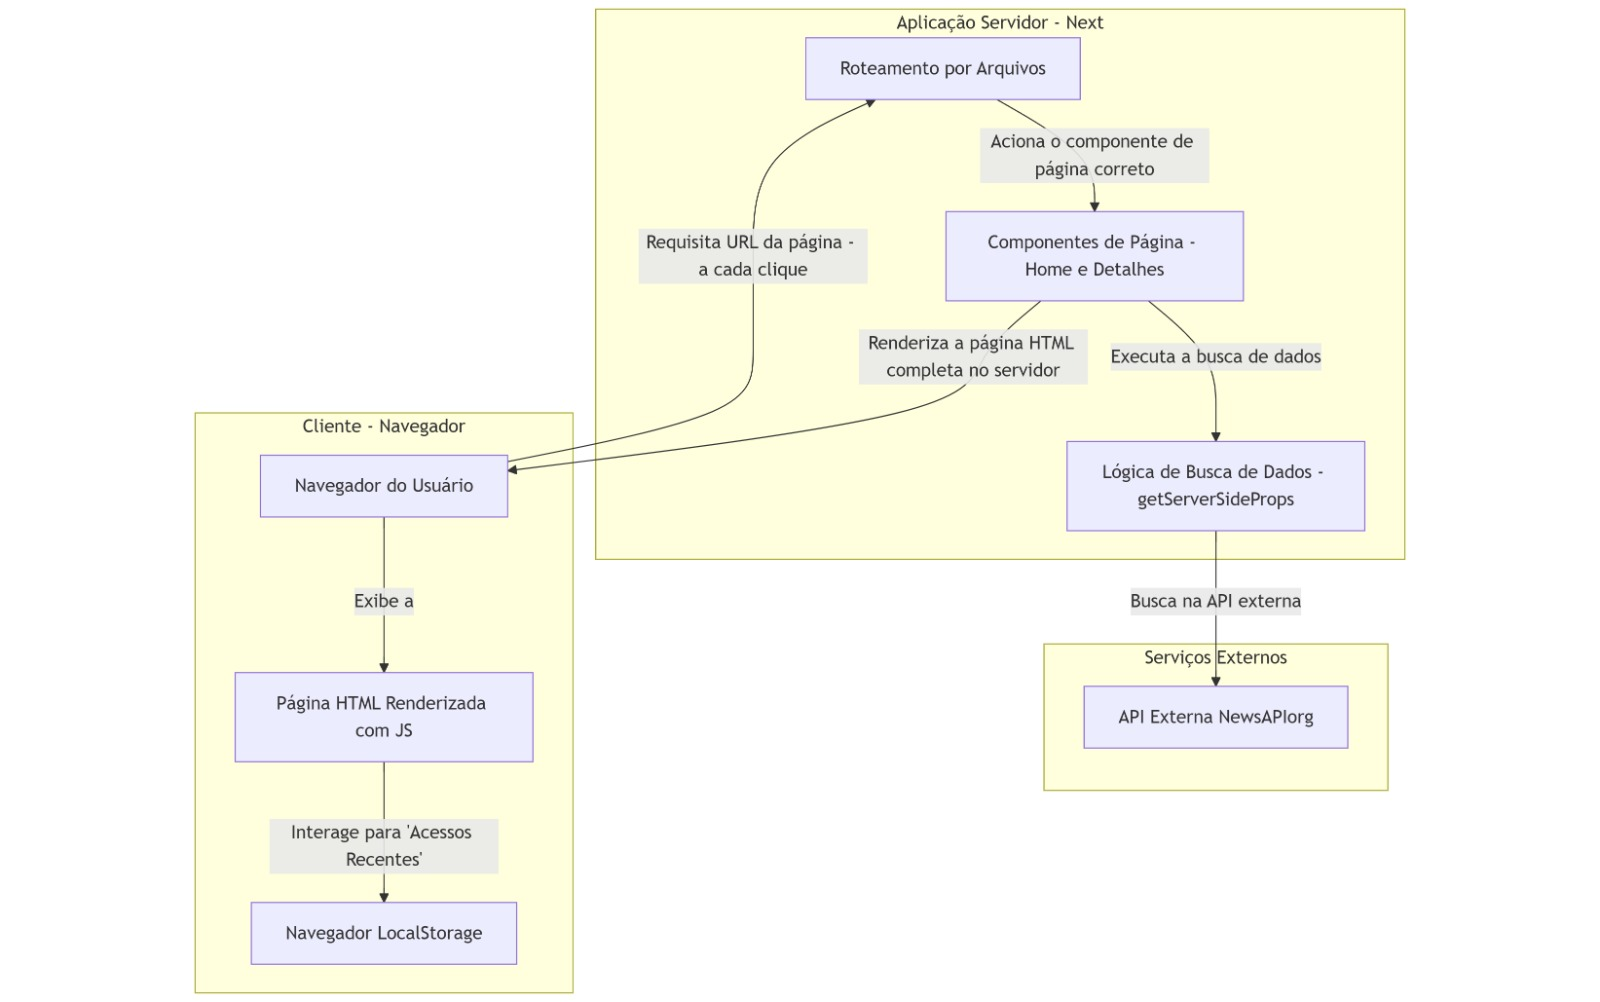
\includegraphics[width=1\textwidth]{media/component-diagram-next.jpeg}
  \legend{Fonte: os autores.}
  \label{fig:component-diagram-next}
\end{figure}


\subsection{CSR/SPA - Fluxo e Arquitetura}
\label{subsec:csr-spa}

Na abordagem \acrfull{csr} com \acrfull{spa}, o carregamento inicial envia um HTML mínimo e um pacote JavaScript que contém toda a lógica da aplicação. A partir daí, a navegação e renderização são executadas no navegador, sem recarregar a página.

\begin{itemize}
  \item O \textbf{usuário} acessa o site;
  \item O navegador baixa o \textbf{bundle React} e monta a interface inicial;
  \item O \textbf{gerenciador de estado} solicita dados à \textbf{NewsAPI};
  \item A interface é atualizada dinamicamente com os dados recebidos;
  \item Ao navegar, o \textbf{roteador do React} altera a URL e renderiza novos componentes;
  \item Dados podem ser lidos ou salvos no \textbf{LocalStorage}.
\end{itemize}

A Figura \ref{fig:sequence-diagram-csr} descreve como o navegador processa as interações: primeiro carrega a aplicação, depois solicita dados conforme necessário e atualiza a interface sem recarregar a página, garantindo uma navegação contínua.

\begin{figure}[H]
  \centering
  \caption{Diagrama de sequência - \acrshort{csr}/\acrshort{spa}}
  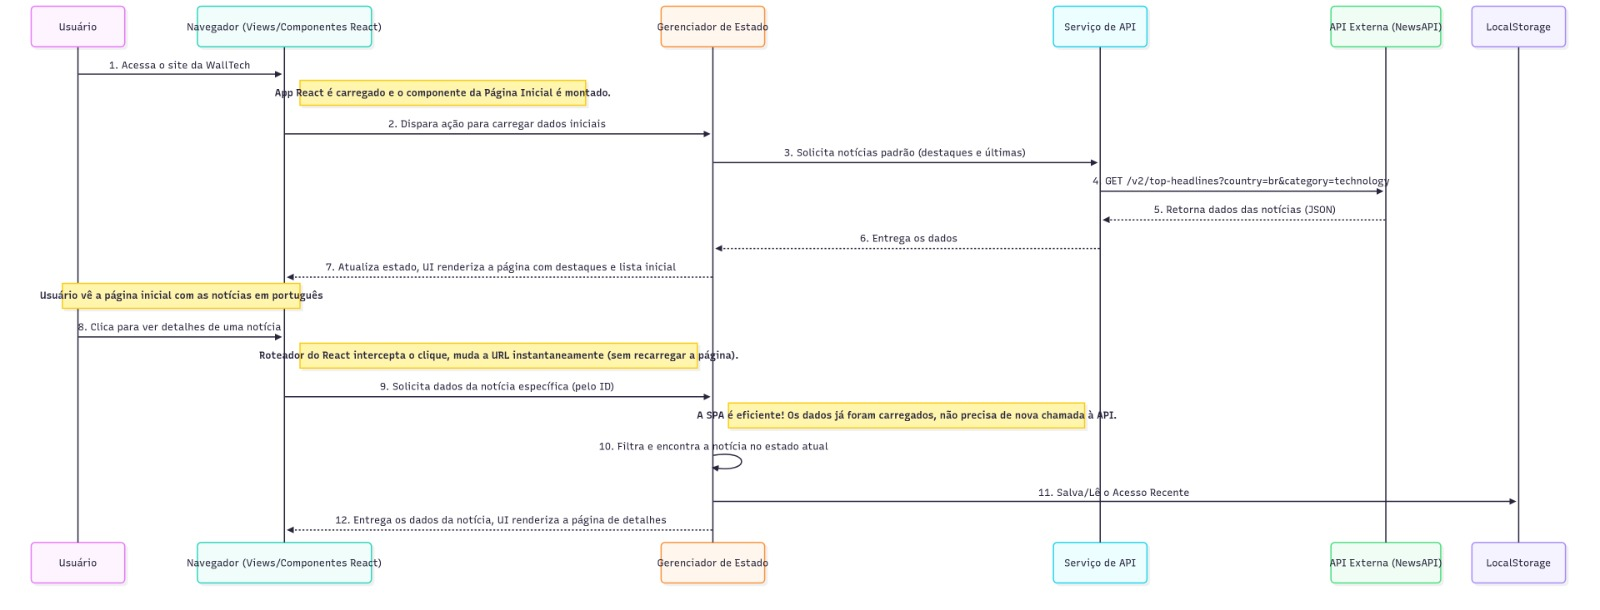
\includegraphics[width=1\textwidth]{media/wall_tech_detail_sequence_diagram.jpeg}
  \legend{Fonte: os autores.}
  \label{fig:sequence-diagram-csr}
\end{figure}


A Figura \ref{fig:component-diagram-react} mostra que, nessa arquitetura, o navegador concentra toda a lógica de renderização. O \textbf{Roteador React} decide quais componentes de página serão exibidos, enquanto o \textbf{Gerenciador de Estado} controla o fluxo de dados entre a interface e a \textbf{NewsAPI}.

\begin{figure}[H]
  \centering
  \caption{Diagrama de Componentes - \acrshort{spa} (React)}
  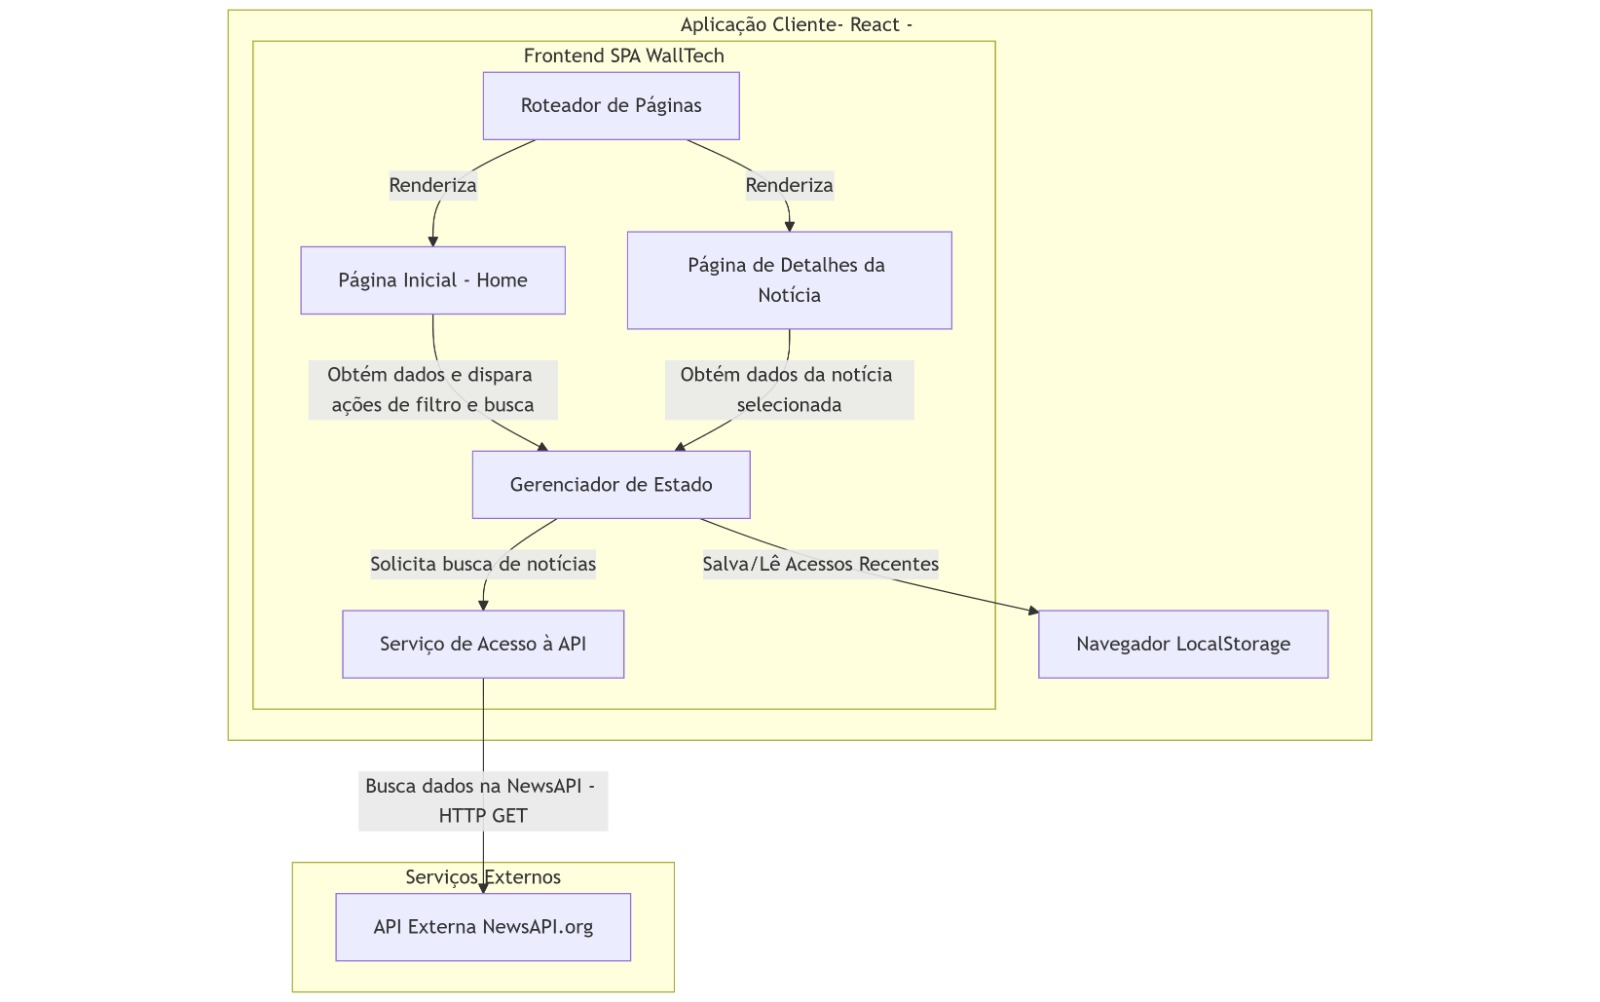
\includegraphics[width=1\textwidth]{media/component-diagram-react.jpeg}
  \legend{Fonte: os autores.}
  \label{fig:component-diagram-react}
\end{figure}



\section{Implementação}
\label{sec:implementacao}

Esta seção descreve o conjunto de tecnologias, bibliotecas e ferramentas que são empregadas para a construção das duas versões do sistema de prova de conceito, detalhando a fundamentação para a escolha de cada componente do ecossistema de desenvolvimento. O gerenciamento do código-fonte e do ciclo de vida do projeto é realizado com o sistema de controle de versão \textbf{Git} e a plataforma de hospedagem \textbf{GitHub}, conforme as práticas descritas na Seção~\ref{sec:git-github}.

Ambas as implementações consomem dados da mesma fonte externa, a \textbf{News API}, uma \acrshort{api} RESTful que fornece o conteúdo jornalístico para a aplicação, como detalhado na Seção~\ref{sec:news-api}. Para garantir a consistência visual e a qualidade da interface entre as duas arquiteturas, utiliza-se a biblioteca de componentes \textbf{shadcn/ui}, que oferece um conjunto de componentes acessíveis e personalizáveis, conforme apresentado na Seção~\ref{sec:ferramentas-modernas}.

\subsection{Implementação da Aplicação SPA}
\label{ssec:implementacao_spa}

A implementação da \acrfull{spa} é desenvolvida utilizando a biblioteca \textbf{React} na sua versão 18. O React é uma biblioteca JavaScript declarativa, mantida pela Meta, focada na construção de interfaces de usuário a partir de componentes reutilizáveis. Sua adoção neste projeto se dá por sua vasta popularidade no mercado e ao seu paradigma de componentização, que facilita a criação de UIs modulares e de fácil manutenção \cite{react2025}. A eficiência da renderização é otimizada pelo uso de um DOM Virtual, um conceito central da biblioteca que minimiza as manipulações diretas no navegador.

Para a estruturação inicial do projeto e o gerenciamento do ambiente de desenvolvimento, utiliza-se a ferramenta de \textit{build} \textbf{Vite}. O Vite é um ecossistema de desenvolvimento frontend moderno que oferece um servidor de desenvolvimento com recarregamento rápido (\textit{Hot Module Replacement}) e um processo de compilação (\textit{build}) otimizado, que resulta em pacotes de produção menores e mais eficientes \cite{vite_docs}.

O roteamento no lado do cliente, uma característica fundamental da arquitetura SPA, implementa-se com a biblioteca \textbf{React Router}. Trata-se da solução padrão para navegação em aplicações React, que possibilita a criação de uma experiência de usuário fluida e sem recarregamentos de página ao manipular a \acrshort{api} de Histórico do navegador \cite{react_router_docs}. A comunicação com a News API é realizada por meio da \acrshort{api} \texttt{fetch}, nativa dos navegadores modernos.

\subsection{Implementação da Aplicação MPA}
\label{ssec:implementacao_mpa}

A implementação da \acrfull{mpa}, com foco em \acrfull{ssr}, é desenvolvida com o \emph{framework} \textbf{Next.js} na versão 14. O Next.js é um meta-framework baseado em React, mantido pela Vercel, que se posiciona como uma solução completa para a construção de aplicações web de produção. Sua escolha para este estudo de caso justifica-se por ser a principal referência de mercado para a implementação de \acrshort{ssr} no ecossistema React, oferecendo uma estrutura robusta e opinativa \cite{nextjs2024}.

O \emph{framework} opera sobre um ambiente \textbf{Node.js}, o que permite a execução de código JavaScript no lado do servidor \cite{nodejs2025}. Essa capacidade é a base da renderização no servidor, onde o Next.js utiliza funções específicas, como a \texttt{getServerSideProps}, para buscar dados de fontes externas e pré-renderizar o HTML completo de uma página antes de enviá-la ao navegador. Além disso, o Next.js implementa um sistema de roteamento baseado no sistema de arquivos, onde a estrutura de diretórios da pasta \texttt{pages} define automaticamente as rotas da aplicação, simplificando a configuração e a manutenção do projeto.